
\special{dvipdfmx:config z 0} %取消PDF压缩,加快速度,最终版本生成的时候最好把这句话注释掉

\documentclass[11pt,a4paper,UTF8]{book}

\usepackage{verbatim}
\usepackage[T1]{fontenc}
\usepackage[utf8]{inputenc}
\usepackage{authblk}

\usepackage{fontspec}                  %引入字体设置宏包
\setmainfont{Times New Roman}             %设置英文正文字体
% Courier New
% Book Antique
\setsansfont{Arial}                    %英文无衬线字体
\setmonofont{Courier New}              %英文等宽字体

\usepackage{ctex} %导入中文包
%\usepackage{ulem}
\usepackage{tocvsec2}


\usepackage{tabularx}
\usepackage{longtable}
\usepackage{booktabs}
\usepackage{multirow}
\usepackage{bbding}
\usepackage{float}
\usepackage{xspace}
\usepackage[none]{hyphenat}
\usepackage{pgffor}

\usepackage{graphicx}
\usepackage{subfigure}
\usepackage{pifont}

\usepackage{hyperref}  %制作pdf的目录
\usepackage{subfiles} %使用多文件方式进行

\usepackage{geometry} %设置页边距的包
\geometry{left=2.5cm,right=2cm,top=2.54cm,bottom=2.54cm} %设置书籍的页边距

\usepackage{url}
\hypersetup{hidelinks, %去红框
  colorlinks=true,
  allcolors=black,
  pdfstartview=Fit,
  breaklinks=true
}

% 调整itemlist中的行间距
\usepackage{enumitem}
\setenumerate[1]{itemsep=0pt,partopsep=0pt,parsep=\parskip,topsep=5pt}
\setitemize[1]{itemsep=0pt,partopsep=0pt,parsep=\parskip,topsep=5pt}
\setdescription{itemsep=0pt,partopsep=0pt,parsep=\parskip,topsep=5pt}

% 超链接样式设置
\usepackage{hyperref}
\hypersetup{
  colorlinks=true,
  linkcolor=blue,
  filecolor=blue,
  urlcolor=blue,
  citecolor=cyan,
}

\usepackage{indentfirst}

\usepackage{listings}
\usepackage[usenames,dvipsnames,svgnames, x11names]{xcolor}
\usepackage{wallpaper}

\usepackage[most]{tcolorbox}
\tcbuselibrary{breakable, minted, skins}

%https://tex.stackexchange.com/questions/173850/problem-in-adding-a-background-color-in-a-minted-environment
\newtcblisting{shell}{
    listing engine=minted,
    minted language=text,%bash, % 使用text就不会有语法高亮显示
    minted options={autogobble,linenos,breaklines},
    listing only,
    size=title,
    arc=0.3mm,
    breakable,
    enhanced jigsaw,
    colframe=black!50!white,
    boxrule=0.5mm,
    colback=bashcodebg,
    coltext=Black,
    minted options={linenos=false,texcl=true},
}
\definecolor{bashcodebg}{rgb}{0.85,0.85,0.85}

% https://tex.stackexchange.com/questions/304449/combine-minted-and-tcolorbox-for-code-from-file-inputminted
\newcounter{inputPrg}
\newtcblisting[use counter=inputPrg, number format=\arabic]{cpp}{
    listing engine=minted,
    minted language=c++,
    minted options={autogobble,linenos,breaklines},
    listing only,
    size=title,
    arc=0.5mm,
    breakable,
    enhanced jigsaw,
    colframe=black!7!white,
    %coltitle=White,
    boxrule=0.5mm,
    colback=blue!3!white,
    coltext=Black,
    %title=\TwoSymbolsAndText{\faCode}{%
        %    \textbf{Input program \thetcbcounter}\ifthenelse{\equal{#2}{}}{}{\textbf{:} \textit{#2}}%
        %}{\faCode},
    %label=inputPrg:#3
    left=6.5mm,enhanced,
    overlay={\begin{tcbclipinterior}\fill[black!5] (frame.south west)
            rectangle ([xshift=5mm]frame.north west);\end{tcbclipinterior}}
}

\usepackage{tikz}

% URL 正确换行
% https://liam.page/2017/05/17/help-the-url-command-from-hyperref-to-break-at-line-wrapping-point/
\makeatletter
\def\UrlAlphabet{%
  \do\a\do\b\do\c\do\d\do\e\do\f\do\g\do\h\do\i\do\j%
  \do\k\do\l\do\m\do\n\do\o\do\p\do\q\do\r\do\s\do\t%
  \do\u\do\v\do\w\do\x\do\y\do\z\do\A\do\B\do\C\do\D%
  \do\E\do\F\do\G\do\H\do\I\do\J\do\K\do\L\do\M\do\N%
  \do\O\do\P\do\Q\do\R\do\S\do\T\do\U\do\V\do\W\do\X%
  \do\Y\do\Z}
\def\UrlDigits{\do\1\do\2\do\3\do\4\do\5\do\6\do\7\do\8\do\9\do\0}
\g@addto@macro{\UrlBreaks}{\UrlOrds}
\g@addto@macro{\UrlBreaks}{\UrlAlphabet}
\g@addto@macro{\UrlBreaks}{\UrlDigits}
\makeatother

% enable subsubsubsection
% from https://tex.stackexchange.com/练习题/274212/correct-hierarchy-levels-of-pdf-bookmarks-for-custom-section-subsubsubsection
\usepackage[depth=3]{bookmark}
\setcounter{secnumdepth}{3}
\setcounter{tocdepth}{4}
\hypersetup{bookmarksdepth=4}

\makeatletter

\newcommand{\toclevel@subsubsubsection}{4}
\newcounter{subsubsubsection}[subsubsection]

\renewcommand{\thesubsubsubsection}{\thesubsubsection.\arabic{subsubsubsection}}

\newcommand{\subsubsubsection}{\@startsection{subsubsubsection}{4}{\z@}%
  {-3.25ex\@plus -1ex \@minus -.2ex}%
  {1.5ex \@plus .2ex}%
  {\normalfont\normalsize\bf\bfseries}}

\newcommand*{\l@subsubsubsection}{\@dottedtocline{4}{11em}{5em}}

\newcommand{\subsubsubsectionmark}[1]{}
\makeatother


\ExplSyntaxOn

% Setup enumerate, itemize and description
\setenumerate  { nosep }
\setitemize    { nosep }
\setdescription{ nosep }

% Setup minted
\setminted { obeytabs, tabsize=2, breaklines=true, fontsize=\footnotesize}

% Def \filename
\NewDocumentCommand { \filename } { m }
{ \noindent  \hspace*{\fill} \\ \textit { #1 } \vspace*{ -1ex } \nopagebreak[4] }

% Def \mySamllsection
\NewDocumentCommand { \mySamllsection } { m }
{\vspace{ 0.2cm } \noindent \textbf { #1 } \vspace*{ 0.05cm } \nopagebreak[4] }

\NewDocumentCommand { \myGraphic } { mmm }
{
  \begin{center}
    \includegraphics[width={#1}\textwidth]{#2}\\
    {#3}
  \end{center}
}

% Def \inlcpp
\NewDocumentCommand { \inlcpp }   { m }
{ \mintinline { cpp } { #1 } }

% Def cpp environment
%\NewDocumentEnvironment { cpp } { }
%{ \VerbatimEnvironment
%  \begin { minted } [ linenos=true, frame=single ] { cpp } }
%{ \end   { minted } }

% Def cmake environment
\NewDocumentEnvironment { cmake } { }
{ \VerbatimEnvironment
  \begin { minted } [ linenos=true, frame=single ] { cmake } }
{ \end   { minted } }

\NewDocumentEnvironment { myNotic } { m }
{ %\hspace*{\fill} \\
  \begin { tcolorbox } [ breakable,colback = blue!5!white, colframe=blue!55!black ,title={#1}] }
{ \end   { tcolorbox } }

\NewDocumentEnvironment { myTip } { m }
{ %\hspace*{\fill} \\
  \begin { tcolorbox } [ breakable,colback = green!5!white, colframe=green!45!black ,title={#1}] }
{ \end   { tcolorbox } }

\NewDocumentEnvironment { myWarning } { m }
{ %\hspace*{\fill} \\
  \begin { tcolorbox } [ breakable,colback=red!5!white,colframe=red!55!black,title={#1}] }
{ \end   { tcolorbox } }

\NewDocumentCommand { \mySubsubsection } { mm }
{
\subsubsection*{\zihao{3} {#1} \hspace{0.2cm}{#2}}
\addcontentsline{toc}{subsubsection}{{#1}\hspace{0.2cm}{#2}}
}

\NewDocumentCommand { \mySubsectionNoFile } { mm }
{
\subsection*{\zihao{3}{#1}\hspace{0.2cm}{#2}}
\addcontentsline{toc}{subsection}{{#1}\hspace{0.2cm}{#2}}
}

\NewDocumentCommand { \mySubsection } { mmm }
{
\subsection*{\zihao{3}{#1}\hspace{0.2cm}{#2}}
\addcontentsline{toc}{subsection}{{#1}\hspace{0.2cm}{#2}}
\subfile{{#3}}
}

\NewDocumentCommand { \mySectionNoHeadImage } { mmm }
{
\color{black}
\pagecolor{white}
\section*{\zihao{2}{#1}\hspace{0.5cm}{#2}}
\addcontentsline{toc}{section}{{#1}\hspace{0.5cm}{#2}}
\subfile{{#3}}
}

\NewDocumentCommand { \CXXTwentythreeLogo } { mm }
{
\noindent
\begin{picture}(0,0)
\put({#1},{#2}){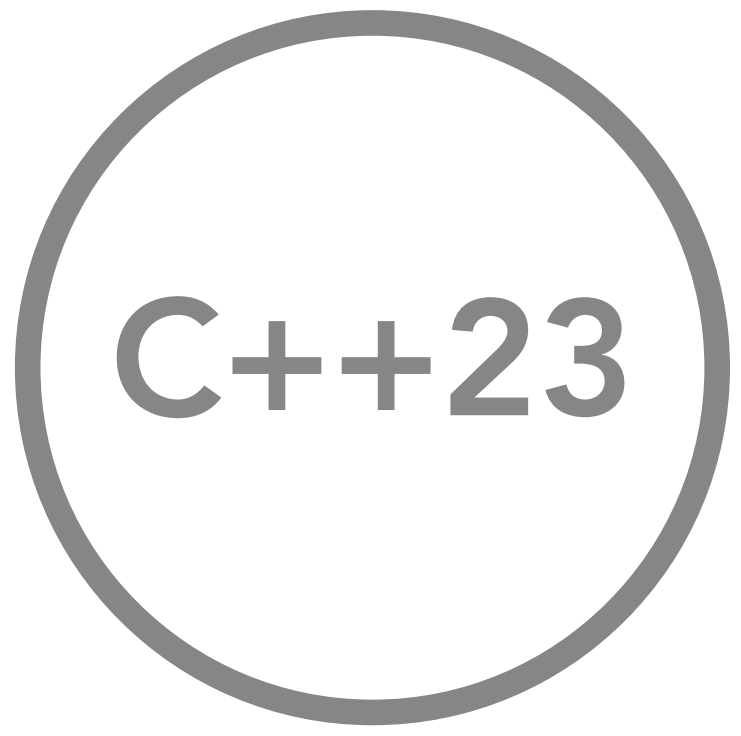
\includegraphics[width=0.07\textwidth]{images/C++23-sign.png}}
\end{picture}
}

\NewDocumentCommand { \mySection } { mmm }
{
\ThisULCornerWallPaper{1.0}{images/section-header.png}
\section*{\zihao{2}{#1}\hspace{0.5cm}{#2}}
\addcontentsline{toc}{section}{{#1}\hspace{0.5cm}{#2}}
\subfile{{#3}}
}

\NewDocumentCommand { \myPart } { mmm }
{
\ThisCenterWallPaper{1.15}{images/section-background.png}
\section*{\zihao{2}{#1}\hspace{0.5cm}{#2}}
\addcontentsline{toc}{section}{{#1}\hspace{0.5cm}{#2}}
\subfile{{#3}}
}

% Latex如何在文本模式批量处理下划线
% https://zhuanlan.zhihu.com/p/615108006

\ExplSyntaxOff

\begin{document}
\begin{sloppypar} %latex中一行文字出现溢出问题的解决方法
%\maketitle

\begin{center}
\thispagestyle{empty}
%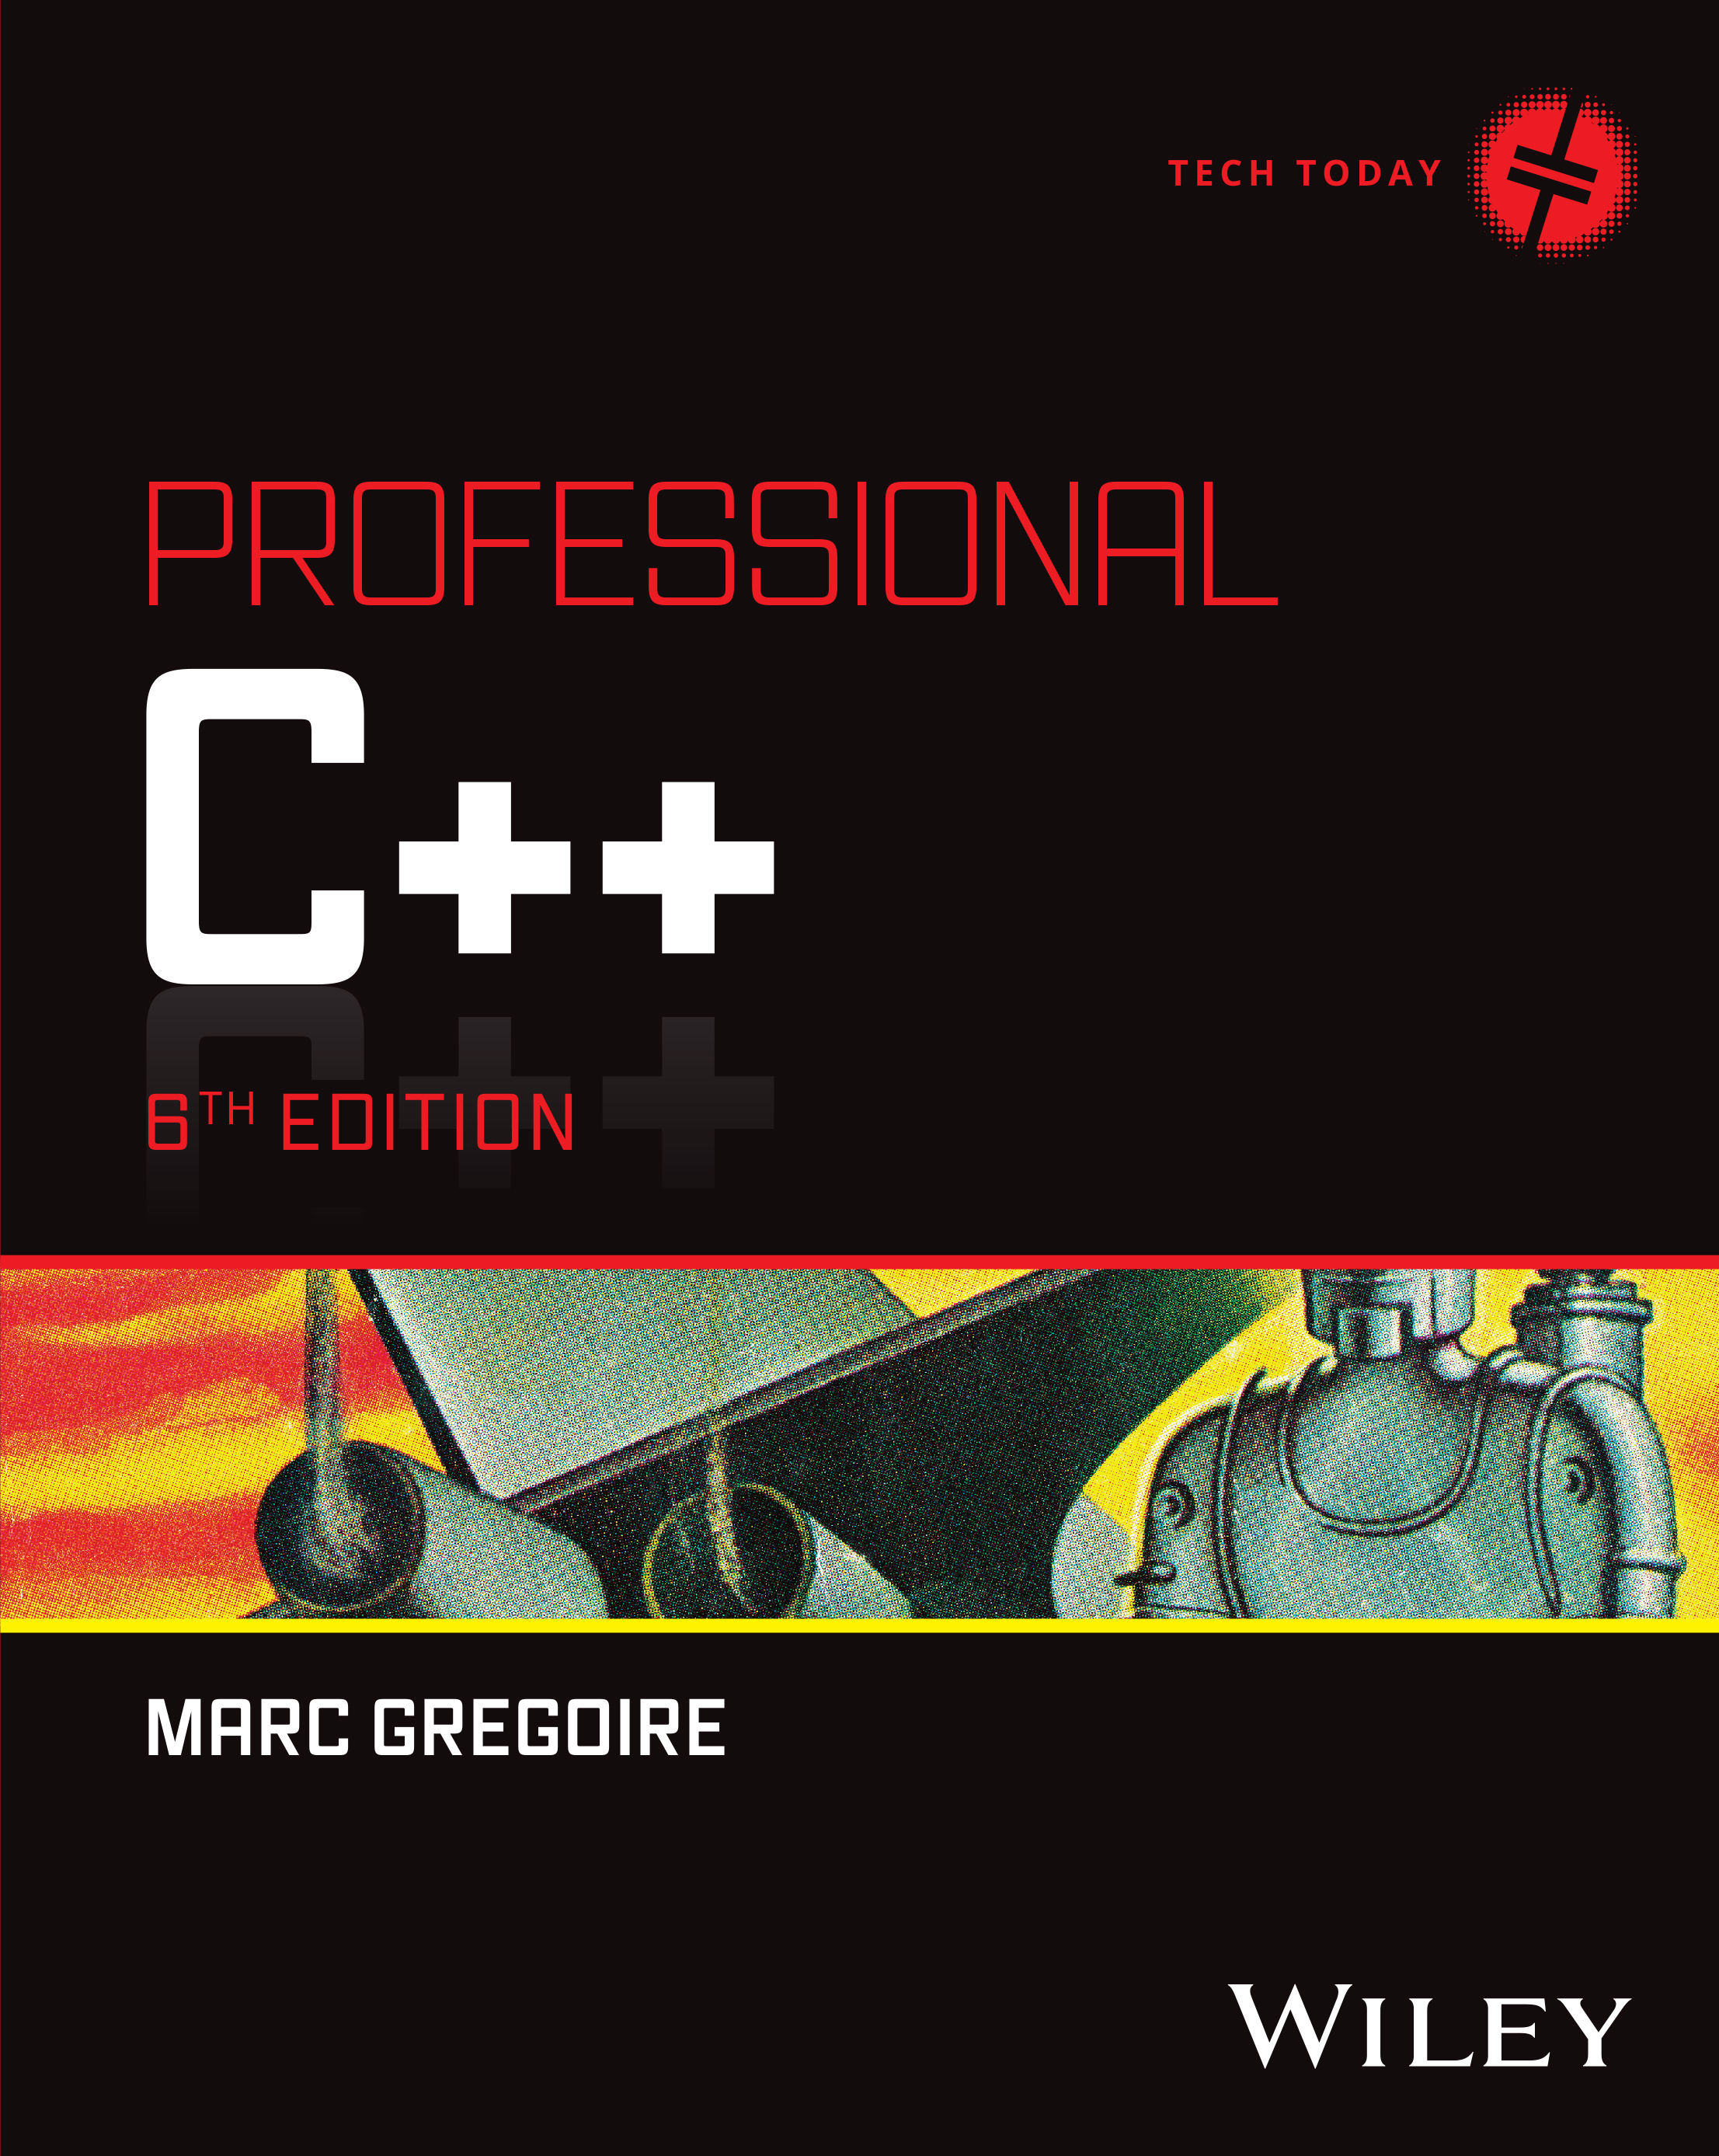
\includegraphics[width=\textwidth,height=\textheight,keepaspectratio]{cover.png}
\begin{tikzpicture}[remember picture, overlay, inner sep=0pt]
\node at (current page.center)
{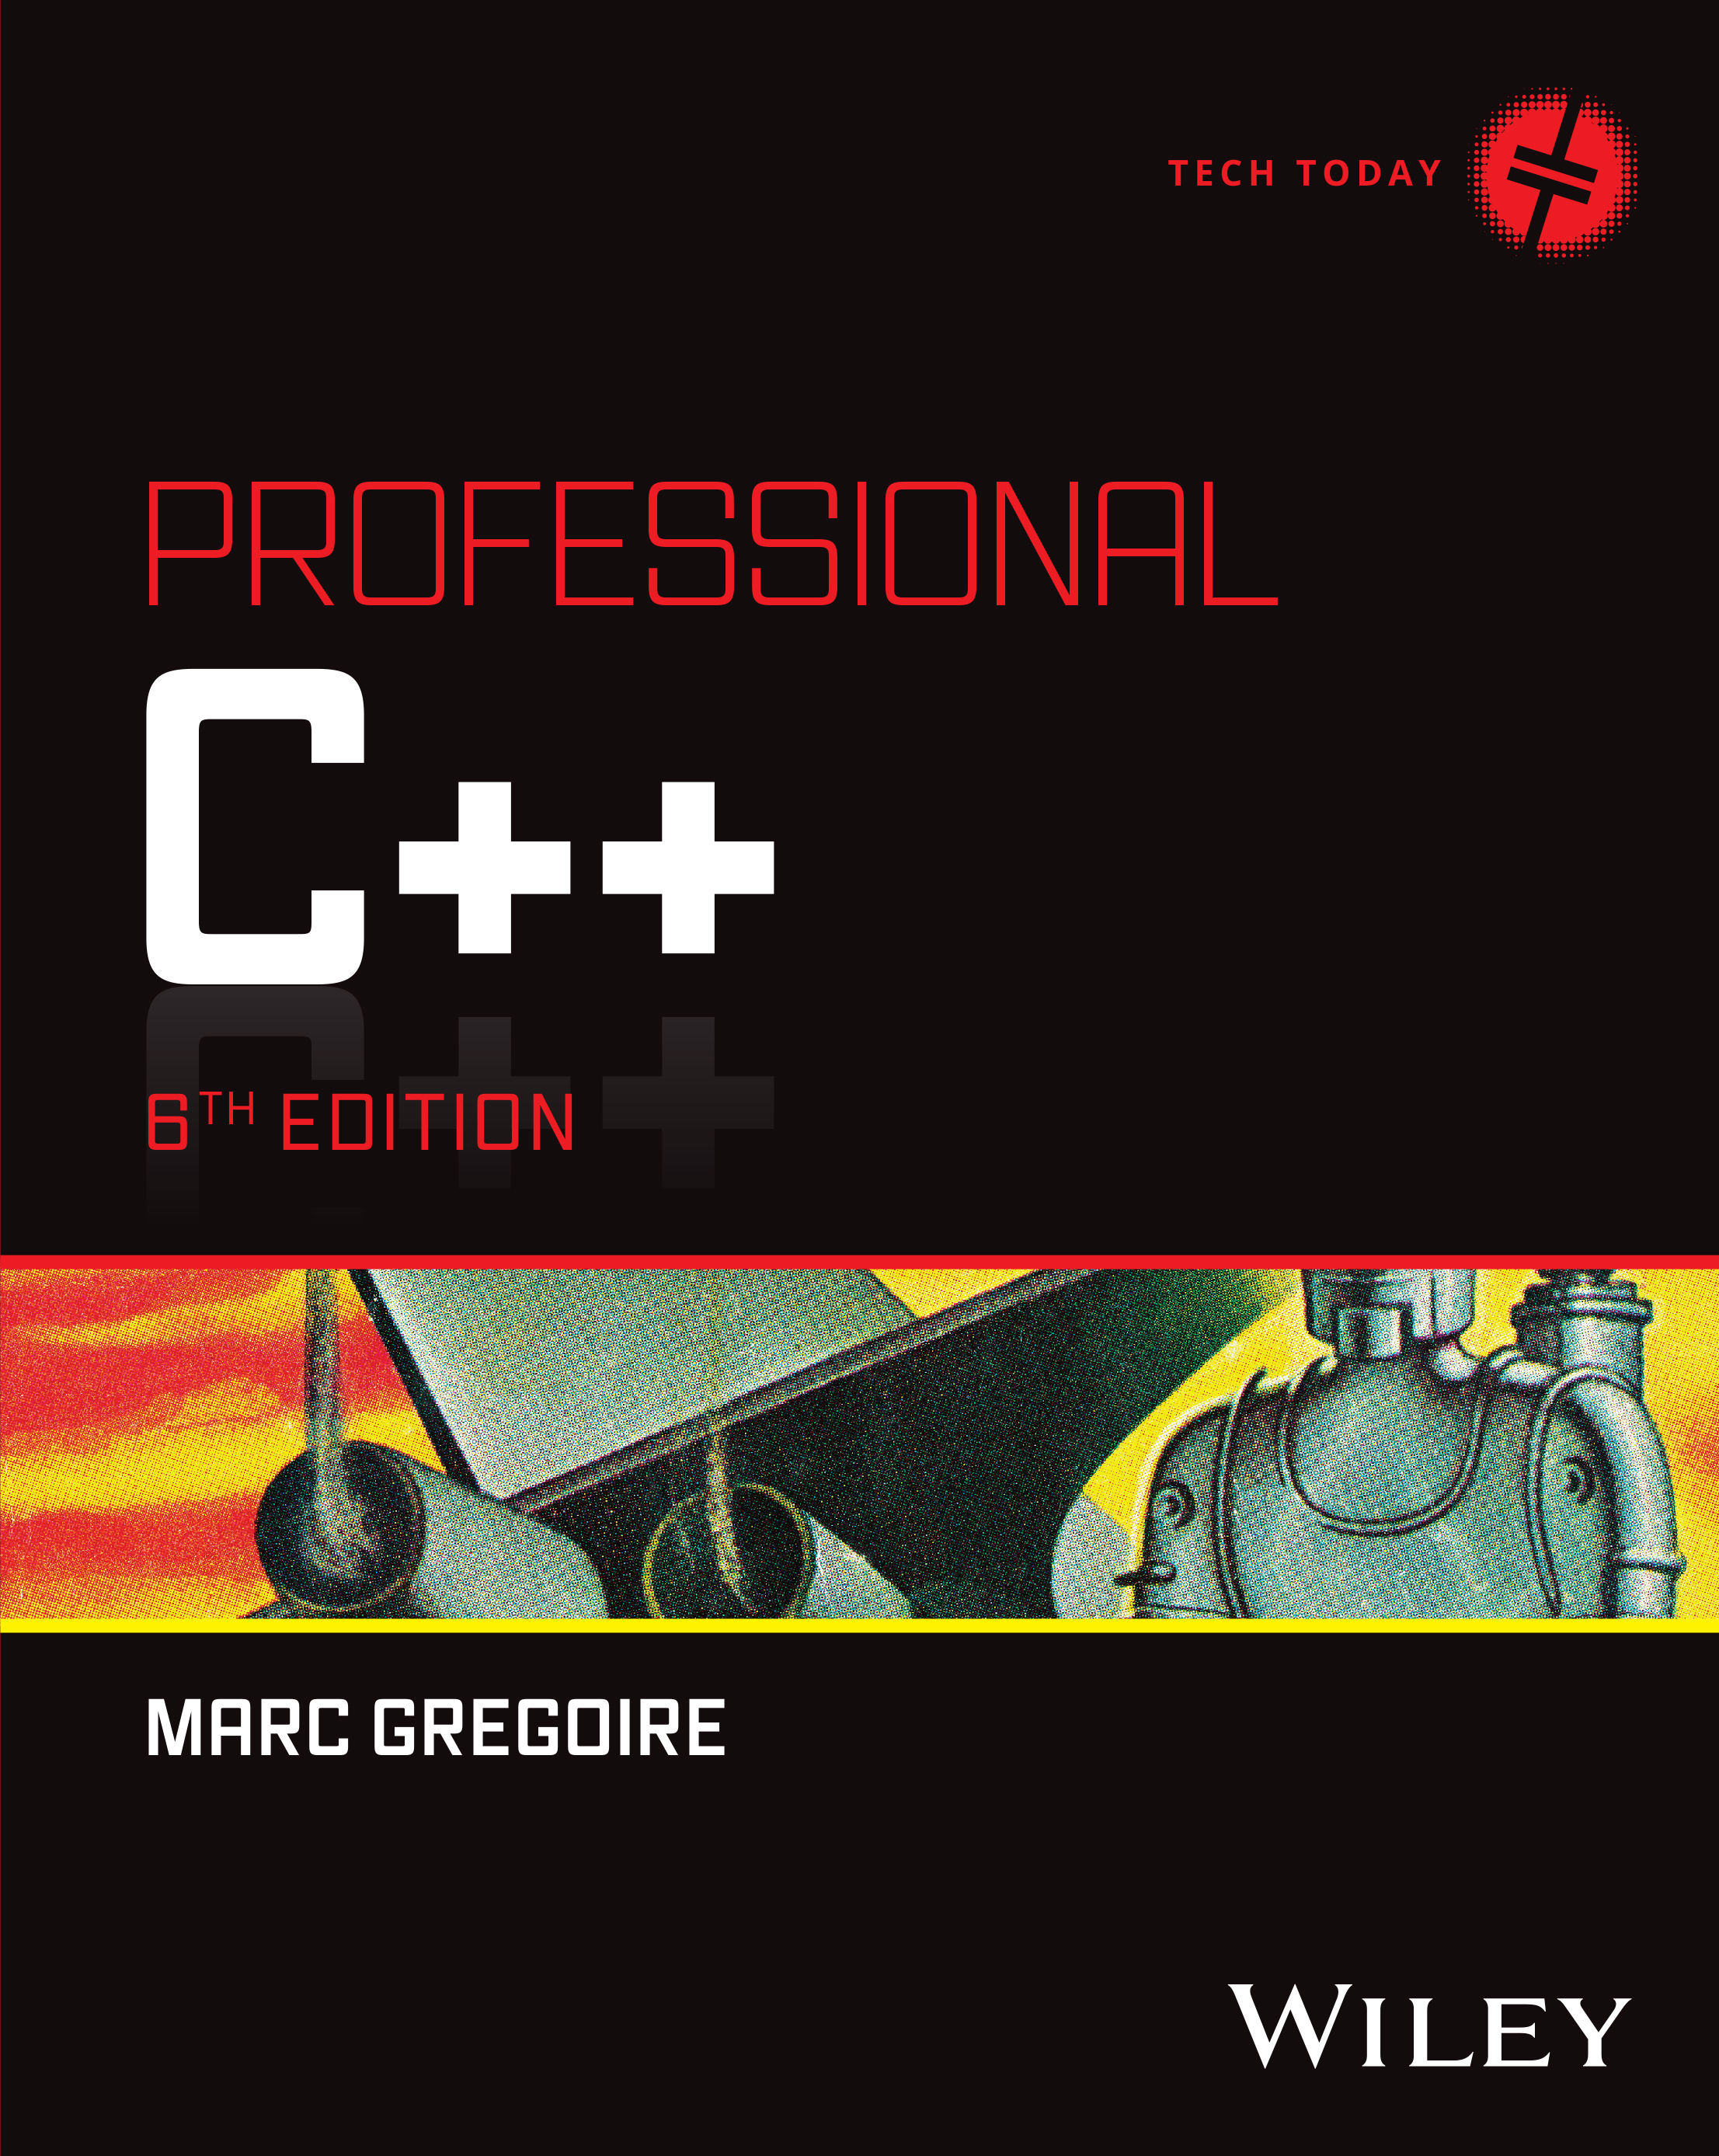
\includegraphics[width=\paperwidth, keepaspectratio=false]{cover.png}};
\end{tikzpicture}
\newpage
\thispagestyle{empty}
\huge
\textbf{Profession C++}
\\[9pt]
{\Large 6th Edition}
\\[9pt]
\normalsize
作者: Marc Gregoire
\\[8pt]
\normalsize
译者:陈晓伟
\\[8pt]
\end{center}

\newpage

\begin{comment}
\pagestyle{empty}
\tableofcontents
\newpage

\setsecnumdepth{section}

\mySectionNoHeadImage{}{关于作者}{content/about-the-author.tex}
\newpage

\mySectionNoHeadImage{}{关于技术编辑}{content/about-the-technical-editor.tex}
\newpage

\mySectionNoHeadImage{}{致谢}{content/acknowledgment.tex}
\newpage

\mySectionNoHeadImage{}{前言}{content/preface.tex}
\newpage

\myPart{第一部分}{Introduction to Professional C++}{content/part1.tex}
\newpage

\mySection{第1章}{A Crash Course in C++ and the Standard Library}{content/part1/chapter1/0.tex}
\mySubsection{1.1.}{C++ Crash Course}{content/part1/chapter1/1.tex}
\mySubsection{1.2.}{Your First Bigger C++ Program}{content/part1/chapter1/2.tex}
\mySubsection{1.3.}{Summary}{content/part1/chapter1/3.tex}
\mySubsection{1.4.}{Exercises}{content/part1/chapter1/4.tex}
\newpage

\mySection{第2章}{Working with Strings and String Views}{content/part1/chapter2/0.tex}
\mySubsection{2.1.}{Dynamic Strings}{content/part1/chapter2/1.tex}
\mySubsection{2.2.}{Formatting And Printing Strings}{content/part1/chapter2/2.tex}
\mySubsection{2.3.}{Summary}{content/part1/chapter2/3.tex}
\mySubsection{2.4.}{Exercises}{content/part1/chapter2/4.tex}
\newpage

\mySection{第3章}{Coding with Style}{content/part1/chapter3/0.tex}
\mySubsection{3.1.}{The Importance Of Looking Good}{content/part1/chapter3/1.tex}
\mySubsection{3.2.}{Documenting Your Code}{content/part1/chapter3/2.tex}
\mySubsection{3.3.}{Decomposition}{content/part1/chapter3/3.tex}
\mySubsection{3.4.}{Naming}{content/part1/chapter3/4.tex}
\mySubsection{3.5.}{Using Language Features With Style}{content/part1/chapter3/5.tex}
\mySubsection{3.6.}{Formatting}{content/part1/chapter3/6.tex}
\mySubsection{3.7.}{Stylistic Challenges}{content/part1/chapter3/7.tex}
\mySubsection{3.8.}{Summary}{content/part1/chapter3/8.tex}
\mySubsection{3.9.}{Exercises}{content/part1/chapter3/9.tex}
\newpage

\myPart{第二部分}{Professional C++ Software Design}{content/part2.tex}
\newpage

\mySection{第4章}{Designing Professional C++ Programs}{content/part2/chapter4/0.tex}
\mySubsection{4.1.}{What Is Programming Design?}{content/part2/chapter4/1.tex}
\mySubsection{4.2.}{The Importance Of Programming Design}{content/part2/chapter4/2.tex}
\mySubsection{4.3.}{Designing For C++}{content/part2/chapter4/3.tex}
\mySubsection{4.4.}{Two Rules For Your Own C++ Designs}{content/part2/chapter4/4.tex}
\mySubsection{4.5.}{Reusing Existing Code}{content/part2/chapter4/5.tex}
\mySubsection{4.6.}{Designing A Chess Program}{content/part2/chapter4/6.tex}
\mySubsection{4.7.}{Summary}{content/part2/chapter4/7.tex}
\mySubsection{4.8.}{Exercises}{content/part2/chapter4/8.tex}
\newpage

\mySection{第5章}{Designing with Classes}{content/part2/chapter5/0.tex}
\mySubsection{5.1.}{Am I Thinking Procedurally?}{content/part2/chapter5/1.tex}
\mySubsection{5.2.}{The Object-oriented Philosophy}{content/part2/chapter5/2.tex}
\mySubsection{5.3.}{Living In A World Of Classes}{content/part2/chapter5/3.tex}
\mySubsection{5.4.}{Class Relationships}{content/part2/chapter5/4.tex}
\mySubsection{5.5.}{Summary}{content/part2/chapter5/5.tex}
\mySubsection{5.6.}{Exercises}{content/part2/chapter5/6.tex}
\newpage

\mySection{第6章}{Designing for Reuse}{content/part2/chapter6/0.tex}
\mySubsection{6.1.}{The Reuse Philosophy}{content/part2/chapter6/1.tex}
\mySubsection{6.2.}{How To Design Reusable Code}{content/part2/chapter6/2.tex}
\mySubsection{6.3.}{Summary}{content/part2/chapter6/3.tex}
\mySubsection{6.4.}{Exercises}{content/part2/chapter6/4.tex}
\newpage

\myPart{第三部分}{C++ Coding the Professional Way}{content/part3.tex}
\newpage

\mySection{第7章}{Memory Management}{content/part3/chapter7/0.tex}
\mySubsection{7.1.}{Working With Dynamic Memory}{content/part3/chapter7/1.tex}
\mySubsection{7.2.}{Array-Pointer Duality}{content/part3/chapter7/2.tex}
\mySubsection{7.3.}{Low-level Memory Operations}{content/part3/chapter7/3.tex}
\mySubsection{7.4.}{Common Memory Pitfalls}{content/part3/chapter7/4.tex}
\mySubsection{7.5.}{Smart Pointers}{content/part3/chapter7/5.tex}
\mySubsection{7.6.}{Summary}{content/part3/chapter7/6.tex}
\mySubsection{7.7.}{Exercises}{content/part3/chapter7/7.tex}
\newpage

\mySection{第8章}{Gaining Proficiency with Classes and Objects}{content/part3/chapter8/0.tex}
\mySubsection{8.1.}{Introducing The Spreadsheet Example}{content/part3/chapter8/1.tex}
\mySubsection{8.2.}{Writing Classes}{content/part3/chapter8/2.tex}
\mySubsection{8.3.}{Understanding Object Life Cycles}{content/part3/chapter8/3.tex}
\mySubsection{8.4.}{Summary}{content/part3/chapter8/4.tex}
\mySubsection{8.5.}{Exercises}{content/part3/chapter8/5.tex}
\newpage

\mySection{第9章}{Mastering Classes and Objects}{content/part3/chapter9/0.tex}
\mySubsection{9.1.}{Friends}{content/part3/chapter9/1.tex}
\mySubsection{9.2.}{Dynamic Memory Allocation In Objects}{content/part3/chapter9/2.tex}
\mySubsection{9.3.}{More About Member Functions}{content/part3/chapter9/3.tex}
\mySubsection{9.4.}{Constexpr And Consteval}{content/part3/chapter9/4.tex}
\mySubsection{9.5.}{Different Kinds Of Data Members}{content/part3/chapter9/5.tex}
\mySubsection{9.6.}{Nested Classes}{content/part3/chapter9/6.tex}
\mySubsection{9.7.}{Enumerations Inside Classes}{content/part3/chapter9/7.tex}
\mySubsection{9.8.}{Operator Overloading}{content/part3/chapter9/8.tex}
\mySubsection{9.9.}{Building Stable Interfaces}{content/part3/chapter9/9.tex}
\mySubsection{9.10.}{Summary}{content/part3/chapter9/10.tex}
\mySubsection{9.11.}{Exercises}{content/part3/chapter9/11.tex}
\newpage

\mySection{第10章}{Discovering Inheritance Techniques}{content/part3/chapter10/0.tex}
\mySubsection{10.1.}{Building Classes With Inheritance}{content/part3/chapter10/1.tex}
\mySubsection{10.2.}{Inheritance For Reuse}{content/part3/chapter10/2.tex}
\mySubsection{10.3.}{Respect Your Parents}{content/part3/chapter10/3.tex}
\mySubsection{10.4.}{Inheritance For Polymorphism}{content/part3/chapter10/4.tex}
\mySubsection{10.5.}{Multiple Inheritance}{content/part3/chapter10/5.tex}
\mySubsection{10.6.}{Interesting And Obscure Inheritance Issues}{content/part3/chapter10/6.tex}
\mySubsection{10.7.}{Casts}{content/part3/chapter10/7.tex}
\mySubsection{10.8.}{Summary}{content/part3/chapter10/8.tex}
\mySubsection{10.9.}{Exercises}{content/part3/chapter10/9.tex}
\newpage

\mySection{第11章}{Modules, Header Files, and Miscellaneous Topics}{content/part3/chapter11/0.tex}
\mySubsection{11.1.}{Modules}{content/part3/chapter11/1.tex}
\mySubsection{11.2.}{Preprocessor Directives}{content/part3/chapter11/2.tex}
\mySubsection{11.3.}{Linkage}{content/part3/chapter11/3.tex}
\mySubsection{11.4.}{Header Files}{content/part3/chapter11/4.tex}
\mySubsection{11.5.}{Feature-test Macros For Core Language Features}{content/part3/chapter11/5.tex}
\mySubsection{11.6.}{The Static Keyword}{content/part3/chapter11/6.tex}
\mySubsection{11.7.}{C-style Variable-length Argument Lists}{content/part3/chapter11/7.tex}
\mySubsection{11.8.}{Summary}{content/part3/chapter11/8.tex}
\mySubsection{11.9.}{Exercises}{content/part3/chapter11/9.tex}
\newpage

\mySection{第12章}{Writing Generic Code with Templates}{content/part3/chapter12/0.tex}
\mySubsection{12.1.}{Overview Of Templates}{content/part3/chapter12/1.tex}
\mySubsection{12.2.}{Class Templates}{content/part3/chapter12/2.tex}
\mySubsection{12.3.}{Function Templates}{content/part3/chapter12/3.tex}
\mySubsection{12.4.}{Variable Templates}{content/part3/chapter12/4.tex}
\mySubsection{12.5.}{Concepts}{content/part3/chapter12/5.tex}
\mySubsection{12.6.}{Summary}{content/part3/chapter12/6.tex}
\mySubsection{12.7.}{Exercises}{content/part3/chapter12/7.tex}
\newpage

\mySection{第13章}{Demystifying C++ I/O}{content/part3/chapter13/0.tex}
\mySubsection{13.1.}{Using Streams}{content/part3/chapter13/1.tex}
\mySubsection{13.2.}{String Streams}{content/part3/chapter13/2.tex}
\mySubsection{13.3.}{Span-based Streams}{content/part3/chapter13/3.tex}
\mySubsection{13.4.}{File Streams}{content/part3/chapter13/4.tex}
\mySubsection{13.5.}{Bidirectional I/O}{content/part3/chapter13/5.tex}
\mySubsection{13.6.}{Filesystem Support Library}{content/part3/chapter13/6.tex}
\mySubsection{13.7.}{Summary}{content/part3/chapter13/7.tex}
\mySubsection{13.8.}{Exercises}{content/part3/chapter13/8.tex}
\newpage

\mySection{第14章}{Handling Errors}{content/part3/chapter14/0.tex}
\mySubsection{14.1.}{Errors And Exceptions}{content/part3/chapter14/1.tex}
\mySubsection{14.2.}{Exception Mechanics}{content/part3/chapter14/2.tex}
\mySubsection{14.3.}{Exceptions And Polymorphism}{content/part3/chapter14/3.tex}
\mySubsection{14.4.}{Rethrowing Exceptions}{content/part3/chapter14/4.tex}
\mySubsection{14.5.}{Stack Unwinding And Cleanup}{content/part3/chapter14/5.tex}
\mySubsection{14.6.}{Source Location}{content/part3/chapter14/6.tex}
\mySubsection{14.7.}{Stack Trace}{content/part3/chapter14/7.tex}
\mySubsection{14.8.}{Common Error-handling Issues}{content/part3/chapter14/8.tex}
\mySubsection{14.9.}{Exception Safety Guarantees}{content/part3/chapter14/9.tex}
\mySubsection{14.10.}{Summary}{content/part3/chapter14/10.tex}
\mySubsection{14.11.}{Exercises}{content/part3/chapter14/11.tex}
\newpage

\mySection{第15章}{Overloading C++ Operators}{content/part3/chapter15/0.tex}
\mySubsection{15.1.}{Overview Of Operator Overloading}{content/part3/chapter15/1.tex}
\mySubsection{15.2.}{Overloading The Arithmetic Operators}{content/part3/chapter15/2.tex}
\mySubsection{15.3.}{Overloading The Bitwise And Binary Logical Operators}{content/part3/chapter15/3.tex}
\mySubsection{15.4.}{Overloading The Insertion And Extraction Operators}{content/part3/chapter15/4.tex}
\mySubsection{15.5.}{Overloading The Subscripting Operator}{content/part3/chapter15/5.tex}
\mySubsection{15.6.}{Overloading The Function Call Operator}{content/part3/chapter15/6.tex}
\mySubsection{15.7.}{Overloading The Dereferencing Operators}{content/part3/chapter15/7.tex}
\mySubsection{15.8.}{Writing Conversion Operators}{content/part3/chapter15/8.tex}
\mySubsection{15.9.}{Overloading The Memory Allocation And Deallocation Operators}{content/part3/chapter15/9.tex}
\mySubsection{15.10.}{Overloading User-defined Literal Operators}{content/part3/chapter15/10.tex}
\mySubsection{15.11.}{Summary}{content/part3/chapter15/11.tex}
\mySubsection{15.12.}{Exercises}{content/part3/chapter15/12.tex}
\newpage

\mySection{第16章}{Overview of the C++ Standard Library}{content/part3/chapter16/0.tex}
\mySubsection{16.1.}{Coding Principles}{content/part3/chapter16/1.tex}
\mySubsection{16.2.}{Overview Of The C++ Standard Library}{content/part3/chapter16/2.tex}
\mySubsection{16.3.}{Summary}{content/part3/chapter16/3.tex}
\mySubsection{16.4.}{Exercises}{content/part3/chapter16/4.tex}
\newpage

\mySection{第17章}{Understanding Iterators and the Ranges Library}{content/part3/chapter17/0.tex}
\mySubsection{17.1.}{Iterators}{content/part3/chapter17/1.tex}
\mySubsection{17.2.}{Stream Iterators}{content/part3/chapter17/2.tex}
\mySubsection{17.3.}{Iterator Adapters}{content/part3/chapter17/3.tex}
\mySubsection{17.4.}{Ranges}{content/part3/chapter17/4.tex}
\mySubsection{17.5.}{Summary}{content/part3/chapter17/5.tex}
\mySubsection{17.6.}{Exercises}{content/part3/chapter17/6.tex}
\newpage

\mySection{第18章}{Standard Library Containers}{content/part3/chapter18/0.tex}
\mySubsection{18.1.}{Containers Overview}{content/part3/chapter18/1.tex}
\mySubsection{18.2.}{Sequential Containers}{content/part3/chapter18/2.tex}
\mySubsection{18.3.}{Sequential Views}{content/part3/chapter18/3.tex}
\mySubsection{18.4.}{Container Adapters}{content/part3/chapter18/4.tex}
\mySubsection{18.5.}{Associative Containers}{content/part3/chapter18/5.tex}
\mySubsection{18.6.}{Other Containers}{content/part3/chapter18/6.tex}
\mySubsection{18.7.}{Summary}{content/part3/chapter18/7.tex}
\mySubsection{18.8.}{Exercises}{content/part3/chapter18/8.tex}
\newpage

\mySection{第19章}{Function Pointers, Function Objects, and Lambda Expressions}{content/part3/chapter19/0.tex}
\mySubsection{19.1.}{Function Pointers}{content/part3/chapter19/1.tex}
\mySubsection{19.2.}{Pointers To Member Functions (and Data Members)}{content/part3/chapter19/2.tex}
\mySubsection{19.3.}{Function Objects}{content/part3/chapter19/3.tex}
\mySubsection{19.4.}{Polymorphic Function Wrappers}{content/part3/chapter19/4.tex}
\mySubsection{19.5.}{Lambda Expressions}{content/part3/chapter19/5.tex}
\mySubsection{19.6.}{Invokers}{content/part3/chapter19/6.tex}
\mySubsection{19.7.}{Summary}{content/part3/chapter19/7.tex}
\mySubsection{19.8.}{Exercises}{content/part3/chapter19/8.tex}
\newpage

\mySection{第20章}{Mastering Standard Library Algorithms}{content/part3/chapter20/0.tex}
\mySubsection{20.1.}{Overview Of Algorithms}{content/part3/chapter20/1.tex}
\mySubsection{20.2.}{Algorithm Details}{content/part3/chapter20/2.tex}
\mySubsection{20.3.}{Summary}{content/part3/chapter20/3.tex}
\mySubsection{20.4.}{Exercises}{content/part3/chapter20/4.tex}
\newpage

\mySection{第21章}{String Localization and Regular Expressions}{content/part3/chapter21/0.tex}
\mySubsection{21.1.}{Localization}{content/part3/chapter21/1.tex}
\mySubsection{21.2.}{Regular Expressions}{content/part3/chapter21/2.tex}
\mySubsection{21.3.}{Summary}{content/part3/chapter21/3.tex}
\mySubsection{21.4.}{Exercises}{content/part3/chapter21/4.tex}
\newpage

\mySection{第22章}{Date and Time Utilities}{content/part3/chapter22/0.tex}
\mySubsection{22.1.}{Compile-time Rational Numbers}{content/part3/chapter22/1.tex}
\mySubsection{22.2.}{Duration}{content/part3/chapter22/2.tex}
\mySubsection{22.3.}{Clock}{content/part3/chapter22/3.tex}
\mySubsection{22.4.}{Time Point}{content/part3/chapter22/4.tex}
\mySubsection{22.5.}{Date}{content/part3/chapter22/5.tex}
\mySubsection{22.6.}{Time Zone}{content/part3/chapter22/6.tex}
\mySubsection{22.7.}{Summary}{content/part3/chapter22/7.tex}
\mySubsection{22.8.}{Exercises}{content/part3/chapter22/8.tex}
\newpage

\mySection{第23章}{Random Number Facilities}{content/part3/chapter23/0.tex}
\mySubsection{23.1.}{C-style Random Number Generation}{content/part3/chapter23/1.tex}
\mySubsection{23.2.}{Random Number Engines}{content/part3/chapter23/2.tex}
\mySubsection{23.3.}{Random Number Engine Adapters}{content/part3/chapter23/3.tex}
\mySubsection{23.4.}{Predefined Engines And Engine Adapters}{content/part3/chapter23/4.tex}
\mySubsection{23.5.}{Generating Random Numbers}{content/part3/chapter23/5.tex}
\mySubsection{23.6.}{Random Number Distributions}{content/part3/chapter23/6.tex}
\mySubsection{23.7.}{Summary}{content/part3/chapter23/7.tex}
\mySubsection{23.8.}{Exercises}{content/part3/chapter23/8.tex}
\newpage

\mySection{第24章}{Additional Vocabulary Types}{content/part3/chapter24/0.tex}
\mySubsection{24.1.}{Variant}{content/part3/chapter24/1.tex}
\mySubsection{24.2.}{Any}{content/part3/chapter24/2.tex}
\mySubsection{24.3.}{Tuple}{content/part3/chapter24/3.tex}
\mySubsection{24.4.}{Optional: Monadic Operations}{content/part3/chapter24/4.tex}
\mySubsection{24.5.}{Expected}{content/part3/chapter24/5.tex}
\mySubsection{24.6.}{Summary}{content/part3/chapter24/6.tex}
\mySubsection{24.7.}{Exercises}{content/part3/chapter24/7.tex}
\newpage

\myPart{第四部分}{Mastering Advanced Features of C++}{content/part4.tex}
\newpage

\mySection{第25章}{Customizing and Extending the Standard Library}{content/part4/chapter25/0.tex}
\mySubsection{25.1.}{Allocators}{content/part4/chapter25/1.tex}
\mySubsection{25.2.}{Extending The Standard Library}{content/part4/chapter25/2.tex}
\mySubsection{25.3.}{Summary}{content/part4/chapter25/3.tex}
\mySubsection{25.4.}{Exercises}{content/part4/chapter25/4.tex}
\newpage

\mySection{第26章}{Advanced Templates}{content/part4/chapter26/0.tex}
\mySubsection{26.1.}{More About Template Parameters}{content/part4/chapter26/1.tex}
\mySubsection{26.2.}{Class Template Partial Specialization}{content/part4/chapter26/2.tex}
\mySubsection{26.3.}{Emulating Function Partial Specialization With Overloading}{content/part4/chapter26/3.tex}
\mySubsection{26.4.}{Template Recursion}{content/part4/chapter26/4.tex}
\mySubsection{26.5.}{Variadic Templates}{content/part4/chapter26/5.tex}
\mySubsection{26.6.}{Metaprogramming}{content/part4/chapter26/6.tex}
\mySubsection{26.7.}{Summary}{content/part4/chapter26/7.tex}
\mySubsection{26.8.}{Exercises}{content/part4/chapter26/8.tex}
\newpage

\mySection{第27章}{Multithreaded Programming with C++}{content/part4/chapter27/0.tex}
\mySubsection{27.1.}{Introduction}{content/part4/chapter27/1.tex}
\mySubsection{27.2.}{Threads}{content/part4/chapter27/2.tex}
\mySubsection{27.3.}{Atomic Operations Library}{content/part4/chapter27/3.tex}
\mySubsection{27.4.}{Mutual Exclusion}{content/part4/chapter27/4.tex}
\mySubsection{27.5.}{Condition Variables}{content/part4/chapter27/5.tex}
\mySubsection{27.6.}{Latches}{content/part4/chapter27/6.tex}
\mySubsection{27.7.}{Barriers}{content/part4/chapter27/7.tex}
\mySubsection{27.8.}{Semaphores}{content/part4/chapter27/8.tex}
\mySubsection{27.9.}{Futures}{content/part4/chapter27/9.tex}
\mySubsection{27.10.}{Example: Multithreaded Logger Class}{content/part4/chapter27/10.tex}
\mySubsection{27.11.}{Thread Pools}{content/part4/chapter27/11.tex}
\mySubsection{27.12.}{Coroutines}{content/part4/chapter27/12.tex}
\mySubsection{27.13.}{Threading Design And Best Practices}{content/part4/chapter27/13.tex}
\mySubsection{27.14.}{Summary}{content/part4/chapter27/14.tex}
\mySubsection{27.15.}{Exercises}{content/part4/chapter27/15.tex}
\newpage

\myPart{第五部分}{C++ Software Engineering}{content/part5.tex}
\newpage

\mySection{第28章}{Maximizing Software Engineering Methods}{content/part5/chapter28/0.tex}
\mySubsection{28.1.}{The Need For Process}{content/part5/chapter28/1.tex}
\mySubsection{28.2.}{Software Life Cycle Models}{content/part5/chapter28/2.tex}
\mySubsection{28.3.}{Software Engineering Methodologies}{content/part5/chapter28/3.tex}
\mySubsection{28.4.}{Building Your Own Process And Methodology}{content/part5/chapter28/4.tex}
\mySubsection{28.5.}{Version Control}{content/part5/chapter28/5.tex}
\mySubsection{28.6.}{Summary}{content/part5/chapter28/6.tex}
\mySubsection{28.7.}{Exercises}{content/part5/chapter28/7.tex}
\newpage

\mySection{第29章}{Writing Efficient C++}{content/part5/chapter29/0.tex}
\mySubsection{29.1.}{Overview Of Performance And Efficiency}{content/part5/chapter29/1.tex}
\mySubsection{29.2.}{Language-level Efficiency}{content/part5/chapter29/2.tex}
\mySubsection{29.3.}{Design-level Efficiency}{content/part5/chapter29/3.tex}
\mySubsection{29.4.}{Profiling}{content/part5/chapter29/4.tex}
\mySubsection{29.5.}{Summary}{content/part5/chapter29/5.tex}
\mySubsection{29.6.}{Exercises}{content/part5/chapter29/6.tex}
\newpage

\mySection{第30章}{Becoming Adept at Testing}{content/part5/chapter30/0.tex}
\mySubsection{30.1.}{Quality Control}{content/part5/chapter30/1.tex}
\mySubsection{30.2.}{Unit Testing}{content/part5/chapter30/2.tex}
\mySubsection{30.3.}{Fuzz Testing}{content/part5/chapter30/3.tex}
\mySubsection{30.4.}{Higher-level Testing}{content/part5/chapter30/4.tex}
\mySubsection{30.5.}{Tips For Successful Testing}{content/part5/chapter30/5.tex}
\mySubsection{30.6.}{Summary}{content/part5/chapter30/6.tex}
\mySubsection{30.7.}{Exercises}{content/part5/chapter30/7.tex}
\newpage

\mySection{第31章}{Conquering Debugging}{content/part5/chapter31/0.tex}
\mySubsection{31.1.}{The Fundamental Law Of Debugging}{content/part5/chapter31/1.tex}
\mySubsection{31.2.}{Bug Taxonomies}{content/part5/chapter31/2.tex}
\mySubsection{31.3.}{Avoid Bugs}{content/part5/chapter31/3.tex}
\mySubsection{31.4.}{Plan For Bugs}{content/part5/chapter31/4.tex}
\mySubsection{31.5.}{Debugging Techniques}{content/part5/chapter31/5.tex}
\mySubsection{31.6.}{Summary}{content/part5/chapter31/6.tex}
\mySubsection{31.7.}{Exercises}{content/part5/chapter31/7.tex}
\newpage

\mySection{第32章}{Incorporating Design Techniques and Frameworks}{content/part5/chapter32/0.tex}
\mySubsection{32.1.}{I Can Never Remember How To. . .}{content/part5/chapter32/1.tex}
\mySubsection{32.2.}{There Must Be A Better Way}{content/part5/chapter32/2.tex}
\mySubsection{32.3.}{Object-oriented Frameworks}{content/part5/chapter32/3.tex}
\mySubsection{32.4.}{Summary}{content/part5/chapter32/4.tex}
\mySubsection{32.5.}{Exercises}{content/part5/chapter32/5.tex}
\newpage

\mySection{第33章}{Applying Design Patterns}{content/part5/chapter33/0.tex}
\mySubsection{33.1.}{The Strategy Pattern}{content/part5/chapter33/1.tex}
\mySubsection{33.2.}{The Abstract Factory Pattern}{content/part5/chapter33/2.tex}
\mySubsection{33.3.}{The Factory Method Pattern}{content/part5/chapter33/3.tex}
\mySubsection{33.4.}{Other Factory Patterns}{content/part5/chapter33/4.tex}
\mySubsection{33.5.}{The Adapter Pattern}{content/part5/chapter33/5.tex}
\mySubsection{33.6.}{The Proxy Pattern}{content/part5/chapter33/6.tex}
\mySubsection{33.7.}{The Iterator Pattern}{content/part5/chapter33/7.tex}
\mySubsection{33.8.}{The Observer Pattern}{content/part5/chapter33/8.tex}
\mySubsection{33.9.}{The Decorator Pattern}{content/part5/chapter33/9.tex}
\mySubsection{33.10.}{The Chain Of Responsibility Pattern}{content/part5/chapter33/10.tex}
\mySubsection{33.11.}{The Singleton Pattern}{content/part5/chapter33/11.tex}
\mySubsection{33.12.}{Summary}{content/part5/chapter33/12.tex}
\mySubsection{33.13.}{Exercises}{content/part5/chapter33/13.tex}
\newpage

\mySection{第34章}{Developing Cross-Platform and Cross-Language Applications}{content/part5/chapter34/0.tex}
\mySubsection{34.1.}{Cross-platform Development}{content/part5/chapter34/1.tex}
\mySubsection{34.2.}{Cross-language Development}{content/part5/chapter34/2.tex}
\mySubsection{34.3.}{Summary}{content/part5/chapter34/3.tex}
\mySubsection{34.4.}{Exercises}{content/part5/chapter34/4.tex}
\newpage

\myPart{第六部分}{Appendices}{content/part6.tex}
\newpage

\end{comment}

\mySection{附录A}{C++ Interviews}{content/part6/appendix-A/0.tex}
\mySubsection{A.1.}{Chapter 1: A Crash Course In C++ And The Standard Library}{content/part6/appendix-A/1.tex}
\mySubsection{A.2.}{Chapters 2 And 21: Working With Strings And String Views, And String Localization And Regular Expressions}{content/part6/appendix-A/2.tex}
\mySubsection{A.3.}{Chapter 3: Coding With Style}{content/part6/appendix-A/3.tex}
\mySubsection{A.4.}{Chapter 4: Designing Professional C++ Programschapter 5: Designing With Classes}{content/part6/appendix-A/4.tex}
\mySubsection{A.5.}{Chapter 6: Designing For Reuse}{content/part6/appendix-A/5.tex}
\mySubsection{A.6.}{Chapter 7: Memory Management}{content/part6/appendix-A/6.tex}
\mySubsection{A.7.}{Chapters 8 And 9: Gaining Proficiency With Classes And Objects, And Mastering Classes And Objects}{content/part6/appendix-A/7.tex}
\mySubsection{A.8.}{Chapter 10: Discovering Inheritance Techniques}{content/part6/appendix-A/8.tex}
\mySubsection{A.9.}{Chapter 11: Modules, Header Files, And Miscellaneous Topics}{content/part6/appendix-A/9.tex}
\mySubsection{A.10.}{Chapters 12 And 26: Writing Generic Code With Templates, And Advanced Templates}{content/part6/appendix-A/10.tex}
\mySubsection{A.11.}{Chapter 13: Demystifying C++ I/O}{content/part6/appendix-A/11.tex}
\mySubsection{A.12.}{Chapter 14: Handling Errors}{content/part6/appendix-A/12.tex}
\mySubsection{A.13.}{Chapter 15: Overloading C++ Operators}{content/part6/appendix-A/13.tex}
\mySubsection{A.14.}{Chapters 16–20 And 25: The Standard Library}{content/part6/appendix-A/14.tex}
\mySubsection{A.15.}{Chapter 22: Date And Time Utilities}{content/part6/appendix-A/15.tex}
\mySubsection{A.16.}{Chapter 23: Random Number Facilities}{content/part6/appendix-A/16.tex}
\mySubsection{A.17.}{Chapter 24: Additional Vocabulary Types}{content/part6/appendix-A/17.tex}
\mySubsection{A.18.}{Chapter 27: Multithreaded Programming With C++}{content/part6/appendix-A/18.tex}
\mySubsection{A.19.}{Chapter 28: Maximizing Software Engineering Methods}{content/part6/appendix-A/19.tex}
\mySubsection{A.20.}{Chapter 29: Writing Efficient C++}{content/part6/appendix-A/20.tex}
\mySubsection{A.21.}{Chapter 30: Becoming Adept At Testing}{content/part6/appendix-A/21.tex}
\mySubsection{A.22.}{Chapter 31: Conquering Debugging}{content/part6/appendix-A/22.tex}
\mySubsection{A.23.}{Chapter 32: Incorporating Design Techniques And Frameworks}{content/part6/appendix-A/23.tex}
\mySubsection{A.24.}{Chapter 33: Applying Design Patterns}{content/part6/appendix-A/24.tex}
\mySubsection{A.25.}{Chapter 34: Developing Cross-platform And Crosslanguage Applications}{content/part6/appendix-A/25.tex}
\newpage

\mySection{附录B}{Annotated Bibliography}{content/part6/appendix-B/0.tex}
\mySubsection{B.1.}{C++}{content/part6/appendix-B/1.tex}
\mySubsection{B.2.}{Unified Modeling Language}{content/part6/appendix-B/2.tex}
\mySubsection{B.3.}{Algorithms And Data Structures}{content/part6/appendix-B/3.tex}
\mySubsection{B.4.}{Random Numbersopen-source Software}{content/part6/appendix-B/4.tex}
\mySubsection{B.5.}{Software Engineering Methodology}{content/part6/appendix-B/5.tex}
\mySubsection{B.6.}{Programming Style}{content/part6/appendix-B/6.tex}
\mySubsection{B.7.}{Computer Architecture}{content/part6/appendix-B/7.tex}
\mySubsection{B.8.}{Efficiency}{content/part6/appendix-B/8.tex}
\mySubsection{B.9.}{Testing}{content/part6/appendix-B/9.tex}
\mySubsection{B.10.}{Debugging}{content/part6/appendix-B/10.tex}
\mySubsection{B.11.}{Design Patterns}{content/part6/appendix-B/11.tex}
\mySubsection{B.12.}{Operating Systems}{content/part6/appendix-B/12.tex}
\mySubsection{B.13.}{Multithreaded Programming}{content/part6/appendix-B/13.tex}
\newpage

\mySection{附录C}{Standard Library Header Files}{content/part6/appendix-C/0.tex}
\mySubsection{C.1.}{Containers}{content/part6/appendix-C/1.tex}
\mySubsection{C.2.}{Unified Modeling Language}{content/part6/appendix-C/2.tex}
\mySubsection{C.3.}{Algorithms, Iterators, Ranges, And Allocators}{content/part6/appendix-C/3.tex}
\mySubsection{C.4.}{General Utilitiesmathematical Utilities}{content/part6/appendix-C/4.tex}
\mySubsection{C.5.}{Exceptions}{content/part6/appendix-C/5.tex}
\mySubsection{C.6.}{I/o Streams}{content/part6/appendix-C/6.tex}
\mySubsection{C.7.}{Threading Support Library}{content/part6/appendix-C/7.tex}
\newpage

\mySection{附录D}{Introduction to UML}{content/part6/appendix-D/0.tex}
\mySubsection{D.1.}{Diagram Types}{content/part6/appendix-D/1.tex}
\mySubsection{D.2.}{Class Diagrams}{content/part6/appendix-D/2.tex}
\mySubsection{D.3.}{Interaction Diagrams}{content/part6/appendix-D/3.tex}
\newpage

\end{sloppypar}
\end{document}

